% Opcje klasy 'iithesis' opisane sa w komentarzach w pliku klasy. Za ich pomoca
% ustawia sie przede wszystkim jezyk oraz rodzaj (lic/inz/mgr) pracy.
\documentclass[shortabstract,inz]{iithesis}
\usepackage[utf8]{inputenc}
\usepackage{natbib}
\usepackage{graphicx}
\usepackage{subcaption}
\usepackage{float}
\usepackage[nottoc]{tocbibind}
\usepackage{url}

\polishtitle    {Koncepcja i implementacja systemu do zarządzania budżetem domowym}
\englishtitle   {Concept and implementation of home budget managment system}
\polishabstract {Celem pracy było stworzenie koncepcji i implementacja systemu służącego do zarządzania budżetem domowym. Motywacją do opracowania takiego systemu było dostarczenie prostego i użytecznego rozwiązania pomagającego użytkownikom w prowadzeniu osobistego budżetu. Do zrealizowania tego celu użyto nowoczesnych oraz popularnych technologii i narzędzi, które pomagają w stworzeniu aplikacji dostępnej z poziomu przeglądarki internetowej.}
\englishabstract{The aim of the work was to develop the concept and implementation of hume budget managment system. The motivation of the work was to provide a simple and useful tool }
% w pracach wielu autorow nazwiska mozna oddzielic poleceniem \and
\author         {Mateusz Kmita}
\advisor        {dr inż. Leszek Grocholski}

%%%%% DANE DO STRONY TYTUŁOWEJ
% Niezaleznie od jezyka pracy wybranego w opcjach klasy, tytul i streszczenie
% pracy nalezy podac zarowno w jezyku polskim, jak i angielskim.
% Pamietaj o madrym (zgodnym z logicznym rozbiorem zdania oraz estetyka) recznym
% zlamaniu wierszy w temacie pracy, zwlaszcza tego w jezyku pracy. Uzyj do tego
% polecenia \fmlinebreak.

% w przypadku kilku promotorow, lub koniecznosci podania ich afiliacji, linie
% w ponizszym poleceniu mozna zlamac poleceniem \fmlinebreak
%\date          {}                     % Data zlozenia pracy
% Dane do oswiadczenia o autorskim wykonaniu
%\transcriptnum {300626}                     % Numer indeksu
%\advisorgen    {dr inż. Leszka Grocholskiego} % Nazwisko promotora w dopelniaczu
%%%%%

%%%%% WLASNE DODATKOWE PAKIETY
%
%\usepackage{graphicx,listings,amsmath,amssymb,amsthm,amsfonts,tikz}
%
%%%%% WŁASNE DEFINICJE I POLECENIA
%
%\theoremstyle{definition} \newtheorem{definition}{Definition}[chapter]
%\theoremstyle{remark} \newtheorem{remark}[definition]{Observation}
%\theoremstyle{plain} \newtheorem{theorem}[definition]{Theorem}
%\theoremstyle{plain} \newtheorem{lemma}[definition]{Lemma}
%\renewcommand \qedsymbol {\ensuremath{\square}}
% ...
%%%%%


\begin{document}

%%%%% POCZĄTEK ZASADNICZEGO TEKSTU PRACY

\chapter{Wprowadzenie}
\section{Opis zagadnienia i motywacje autora}
W ramach tej pracy zajmuję się zagadnieniem prowadzenia budżetu domowego, które polega na podziale posiadanych pieniędzy pomiędzy obszary, na które chcemy je przeznaczyć. Z jednej strony budżet domowy wymaga poświęcenia dodatkowego czasu na stworzenie oraz jego regularne prowadzanie. Z drugiej strony możemy w zamian liczyć na większą kontrolę nad stanem naszego portfela. Przy założeniu, że taki budżet prowadzony jest regularnie, mamy wiedzę o tym, ile pieniędzy możemy jeszcze wydać. Może to pozwolić nawet na uniknięcie długów. Osoba prowadząca budżet domowy i historię wydatków może także łatwiej analizować swoje nawyki konsumenckie oraz je poprawiać, aby móc efektywniej zarządzać swoimi pieniędzmi w przyszłości.
\bigbreak
Zdecydowałem się na stworzenie aplikacji, która będzie dostarczała wszystkie wymagane podstawowe funkcjonalności do zrealizowania opisanego wyżej zadania oraz będzie na tyle prosta, aby nowy użytkownik mógł jak najmniejszym kosztem zacząć prowadzić swój budżet domowy. W dalszej części pracy opisałem jakie funkcje udostępnia aplikacja. Następnie skupiłem się na przedstawieniu i uzasadnieniu mojego rozwiązania pod względem technologicznym. W końcowej części pracy podsumowałem zrealizowane zadania oraz podałem przykłady sposobów na dalsze ulepszenie aplikacji.

\section{Przykłady innych rozwiązań}
Użytkownicy zainteresowani tematyką prowadzenia budżetu domowego mają duży wybór dostępnych rozwiązań. Istnieją zarówno aplikacje dostępne przez przeglądarkę, tradycyjne programy i aplikacje na urządzenia mobilne. Wiele programów dostępnych jest jednocześnie na wielu rodzajach urządzeń dla wygody użytkowników. Ja skupiłem się na rozwiązaniach, które dostępne są przez przeglądarkę, gdyż są najbardziej zbliżone do rozwiązania proponowanego przeze mnie.
\subsection{You Need a Budget (YNAB)}
Aplikacja You Need a Budget \citep{ynab} jest dostępna przez przeglądarkę internetową oraz w postaci aplikacji na urządzenia mobilne na systemy operacyjne Android i iOS. Jest to program płatny, który kosztuje 14,99\$ miesięcznie lub 89,99\$ rocznie \cite{ynab-price}. Ideą tej aplikacji jest nie tyle zautomatyzowanie całego procesu zarządzania budżetem i całkowite wyręczenie użytkownika, co nauczenie go jak taki budżet tworzyć, więc aplikacja YNAB wymaga od użytkownika poświęcenia czasu na ręczne tworzenie budżetu. Filozofia tworzenia budżetu domowego w tej aplikacji polega na rozdzieleniu pieniędzy co do grosza na nasze cele. Program ten posiada użyteczną funkcję automatycznego pobierania wydatków z konta bankowego.

\subsection{Mint}
Mint \cite{mint} to darmowy program dostępny przez przeglądarkę internetową oraz jako aplikacja na urządzenia mobilne na systemy operacyjne Android i iOS. Aplikacja dostępna jest za darmo, ale wyświetla użytkownikom reklamy ofert od swoich partnerów biznesowych. To rozwiązanie posiada wiele funkcji automatyzujących cały proces zarządzania budżetem. Automatycznie pobiera wydatki z połączonego konta bankowego i przypisuje je do odpowiednich kategorii. Posiada też dodatkowe funkcje oprócz prowadzenia budżetu takie jak przypominanie o płatnościach za subskrypcje i rachunki lub wysyłanie użytkownikom porad, jak mogą lepiej zarządzać pieniędzmi. Dostępne są także informacje o zdolności kredytowej, funkcje związane z inwestowaniem oraz inne funkcjonalności dotyczące pieniędzy. Mamy więc tutaj więcej funkcji niż w poprzednim rozwiązaniu.

\begin{figure}[h]
\centering
\begin{subfigure}{0.45\textwidth}
    
\includegraphics[width=\textwidth]{mint-screen.jpg}
    \caption{Mint}
    \label{fig:mint}
\end{subfigure}
\hfill
\begin{subfigure}{0.45\textwidth}
    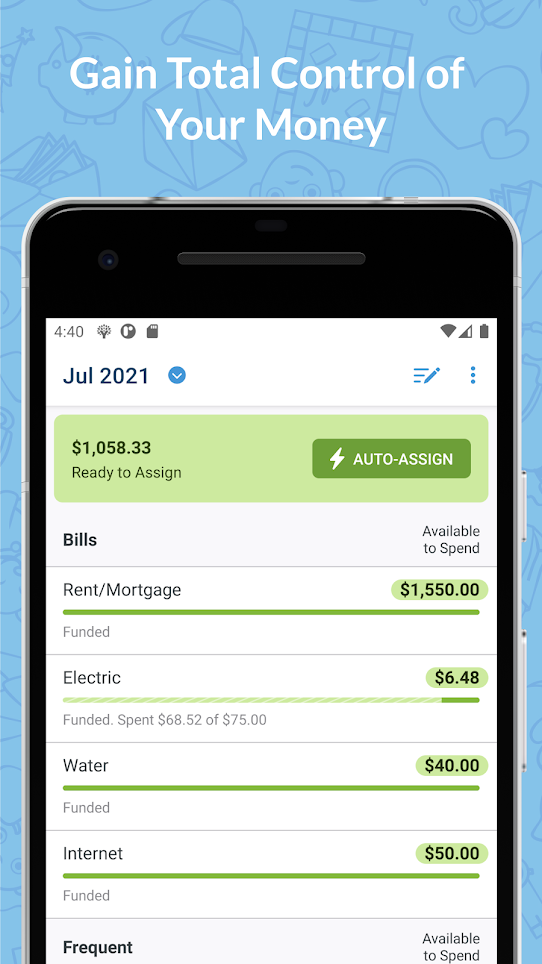
\includegraphics[width=\textwidth]{ynab.png}
    \caption{You Need A Budget}
    \label{fig:ynab}
\end{subfigure}
        
\caption{Inne rozwiązania dotyczące prowadzenia budżetu osobistego}
\label{fig:mint-ynab}
\end{figure}

\chapter{Opis systemu}
\section{Sposób instalacji i dostępu do systemu}
\section{Opis funkcji systemu}
Koncepcja aplikacji polega na założeniu, że użytkownik będzie samodzielnie regularnie rejestrował w aplikacji wszystkie swoje wydatki oraz wpływy oraz ręcznie tworzył budżet rozdzielając pieniądze pomiędzy różne kategorie. Program będzie te informacje zapisywał oraz obliczał środki dostępne w ramach budżetu.

Poniżej wytłumaczyłem podstawowe pojęcia używane w aplikacji.
\begin{itemize}
	\item \textbf{Transakcje} - operacje pieniężne, które są wydatkami lub wpływami z zewnętrznych źródeł. Te operacje mogą wpływać na stan budżetu.
	\item \textbf{Transfery} - operacje pieniężne pomiędzy dwoma różnymi kontami, które nie wpływają na budżet, ale dotyczą przeniesienia środków wewnątrz portfela użytkownika
		\item \textbf{Kategoria transakcji} - podział wszystkich transakcji na różne kategorie dotyczące tej samej dziedziny. Ocena do jakiej kategorii należy transakcja leży całkowicie po stronie użytkownika.
	\item \textbf{Budżet} - budżet to comiesięczny podział wpływów pomiędzy różne kategorie wraz z wydatkami w tym miesiącu oraz informacją o środkach dostępnych jeszcze w ramach każdej z kategorii.

\end{itemize}
\subsection{Zarządzanie kontami}
Użytkownik posiada możliwość podziału swojego portfela na różne konta. Ta funkcja pozwala śledzić ilość pieniędzy ulokowanych w różnych źródłach. Dla wygody użytkownika konta są podzielone pomiędzy cztery różne rodzaje: rozliczeniowe, oszczędnościowe, gotówkę oraz inne. Lista kont wyświetlana jest w panelu nawigacyjnym po lewej stronie ekranu. Możemy stamtąd przejść do listy transakcji lub transferów przypisanych do każdego z kont. Na górze strony będą wtedy wyświetlane informacje o koncie, którego ekran dotyczy. Znajdziemy tam nazwę konta, opis, rodzaj i aktualny stan środków na koncie. Obok tych informacji znajdują się przyciski ``Usuń konto'' oraz ``Edytuj konto'' służące do usuwania konta i edycji danych o nim. Aby dodać nowe konto należy nacisnąć na przycisk "Dodaj konto" w panelu nawigacyjnym. Wyświetla się wtedy formularz, w którym należy podać nazwę i rodzaj konta oraz opcjonalnie opis i początkowy stan tego konta.

\begin{figure}[h]
	\centering
	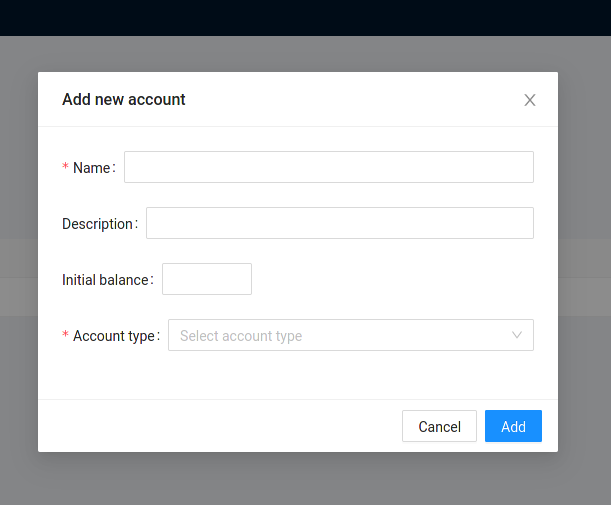
\includegraphics[scale=0.7]{screen-new-account.png}
	\caption{Formularz tworzenia nowego konta}
	\label{fig:screen-new-account}
\end{figure}

\begin{figure}[h]
	\centering
	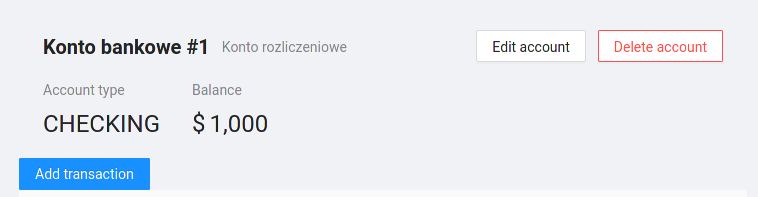
\includegraphics[scale=0.7]{screen-panel-info-konto.png}
	\caption{Widok informacji o koncie}
	\label{fig:screen-account-info}
\end{figure}
\subsection{Wyświetlanie operacji}

\subsection{Rejestrowanie operacji}
Zgodnie z koncepcją aplikacji, użytkownik powinien regularnie rejestrować w programie swoje wydatki, przychody i transfery pieniędzy. Aby to zrobić, należy nacisnąć na przycisk ``Add transaction'' lub ``Add transfer''. Są one widoczne na ekranach transakcji i transferów dla danego konta. Pierwszy z nich służy do zapisywania transakcji, a drugi do zapisywania transferów na danym koncie. Naciśnięcie tych przycisków powoduje wyświetlenie okienka z formularzem. Należy w nim podać dane o operacje. Niektóre pola są wymagane i oznaczone są one znakiem czerwonej gwiazdki. Pozostałe pola są opcjonalne.

\begin{figure}[h]
	\centering
	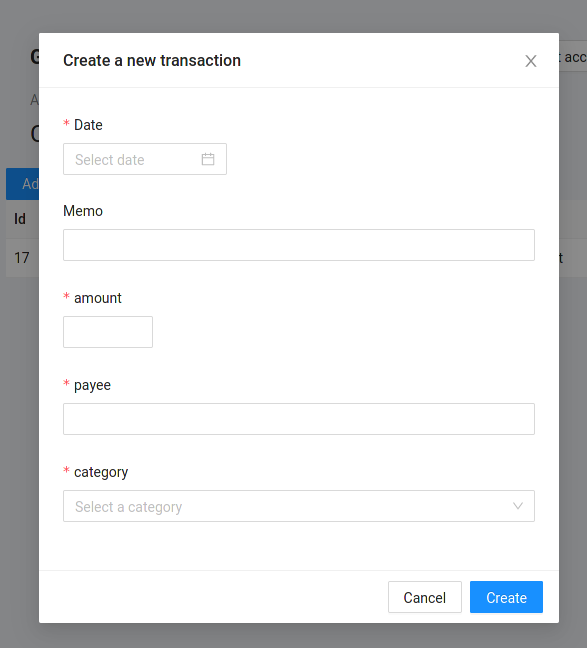
\includegraphics[scale=0.7]{screen-new-transaction-form.png}
	\caption{Formularz dodawania nowej transakcji}
	\label{fig:screen-new-transaction}
\end{figure}

\begin{figure}[h!]
	\centering
	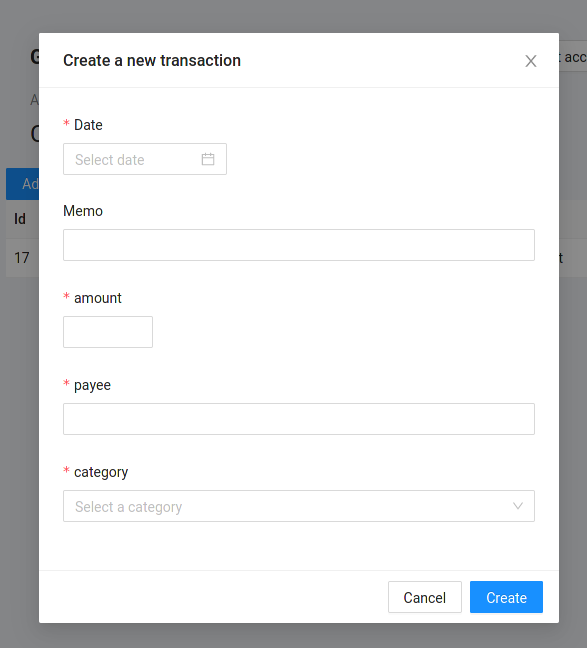
\includegraphics[scale=0.7]{screen-new-transaction-form.png}
	\caption{Formularz dodawania nowego transferu pomiędzy kontami}
	\label{fig:screen-new-transfer}
\end{figure}

\subsection{Wyświetlanie budżetów}
\subsection{Tworzenie budżetów}
\subsection{Wyświetlanie statystyk}


\chapter{Użyte rozwiązania technologiczne}
Program został podzielony na dwie części. Pierwsza z nich to część serwerowa. Odpowiada ona za logikę programu i przechowywanie danych w trwałej pamięci. Druga część to część kliencka. Jej głównym zadaniem jest prezentacja danych otrzymanych od części serwerowej użytkownikowi. Komunikacja między tymi dwiema warstwami odbywa się przez protokół HTTP. W dalszej części tego rozdziału dokładniej opisuję obie te warstwy programu.
\section{Część serwerowa}
Część serwerowa programu została napisana z użyciem języka Java. W kodzie źródłowym możemy wydzielić trzy warstwy. Pierwsza z nich to warstwa dostępu do danych. Ta część programu komunikuje się z bazą danych i tłumaczy jej relacyjny system typów na architekturę obiektową języka Java. Druga warstwa to tzw. warstwa serwisowa. Udostępnia ona główną logikę działania programu i komunikuje się z jednej strony z warstwą dostępu do danych, aby zapisywać informacje w trwałej pamięci, a z drugiej strony udostępnia wyższej warstwie zbiór dostępnych do wykonywania w ramach logiki programu operacji. Tą wyższą warstwą jest warstwa kontrolerów. Kontrolery to obiekty wyspecjalizowane do odbierania żądań ze świata zewnętrznego. Korzystają z warstwy serwisów, aby zlecone żądania wykonać.
Kontrolery udostępniają bezstanowy interfejs API dostępu do programu. Aplikacja stworzona jest z wykorzystaniem architektury Representational State Transfer (REST) \cite{rest} , więc udostępnia zasoby (zasobem jest np. konto, transakcja, budżet), na których można wykonywać operacje zdefiniowane przez protokół HTTP, które powodują zmianę stanu tych zasobów.
\subsection{Spring}
Główną technologią użytą w tworzeniu części serwerowej jest framework Spring \cite{spring}. Jest to obecnie najpopularniejszy framework do tworzenia aplikacji w języku Java \cite{spring-popularity}. Pod nazwą Spring kryje się tak naprawdę wiele różnych bibliotek. Cały framework podzielony jest więc na moduły rozwiązujące różne problemy \cite{spring-modules} takie jak udostępnianie kontenera Inversion of Control (IoC) \citep{ioc}, tworzenie aplikacji internetowych, tworzenie aplikacji dla środowiska rozporoszonego uruchamianych w chmurze, zabezpieczanie aplikacji, dostęp do baz danych i inne. Udostępnianie kontenera IoC jest jedną z głównych funkcji tego frameworka, a implementacja tego wzorca w postaci zasady Dependency Injection jest używana także w mojej aplikacji.

W moim rozwiązaniu użyłem między innymi modułu Spring MVC \cite{spring-mvc}, który używany jest w warstwie prezentacji danych. Dzięki temu rozwiązaniu mogłem z łatwością odczytywać żądania przesyłane do kontrolerów w aplikacji z zewnątrz przez protokół HTTP. Spring MVC bazuje na technologii Servlet API i ułatwia definiowanie zasobów w architekturze REST. Wystarczy stworzyć metody i zdefiniować jakie adresy i metody HTTP mają one obsługiwać. Spring MVC zajmie się za nas niskopoziomowymi kwestiami obsługi żądań takimi jak odbieranie danych, tłumaczenie ich na obiekty języka Java i wysyłanie odpowiedzi.

Aby ułatwić sobie tworzenie aplikacji użyłem także modułu Spring Boot \cite{spring-boot}. Spring Framework wymaga konfiguracji używanych elementów poprzez pliki XML, kod Java lub adnotacje w języku Java \citep{java-annotations}. Twórcy tej biblioteki zauważyli, że większość programistów wybiera przy tworzeniu programów podobne opcje konfiguracji biblioteki Spring. Aby ułatwić z nią pracę, Spring Boot automatyzuje proces konfiguracji, zarówno elementów dotyczących frameworka Spring jak i innych bibliotek, udostępniając zdefiniowane wcześniej konfiguracje tych elementów. Pozwala to o wiele szybciej rozpocząć tworzenie programów nieprzejmując się pisaniem konfiguracji dopóki nie będziemy mieli żadnych specyficznych wymagań. Dzięki temu będziemy mieli mniej powtarzalnego kodu w naszej aplikacji.
\subsection{Schemat bazy danych}
\subsection{Inne technologie użyte w  części serwerowej}
\section{Część kliencka}
\subsection{Biblioteka React}

\chapter{Podsumowanie}
\section{Możliwości dalszej rozbudowy}
%%%%% BIBLIOGRAFIA

\bibliographystyle{unsrt}
\bibliography{bibliography}


\end{document}
